\documentclass[a4paper, 12pt]{article}
% math symbols
\usepackage{amssymb}
\usepackage{amsmath}
\usepackage{mathrsfs}
\usepackage{physsummer}


\usepackage{enumitem}
\usepackage[margin = 2cm]{geometry}

\tolerance = 1000
\emergencystretch = 0.74cm



\pagestyle{empty}
\parindent = 0mm

\begin{document}

\begin{center}
  \Large{\textbf{11 класс.}\\
  \textit{8 октября 2014.}}
\end{center}


\begin{center}
  \Large \textbf{Виртуальные перемещения.}
\end{center}

\large

\task{ Однородная резинка пренебрежимо малой начальной длины при
  растяжении подчиняется закону Гука и имеет жесткость $K$. Материал
  резинки равномерно заряжен, ее полный заряд $Q>0$. Резинку поместили
  в поле двух зарядов $+q$ и $-q$, расположенных на расстоянии $2L$
  друг от друга. Один из концов резинки удерживают посередине между
  зарядами, прикладывая при этом силу $F_1$. Какая сила $F_2$ должна
  быть приложена для удержания второго конца, если он находится на
  расстоянии $L$ справа от заряда $+q$? Взаимодействием зарядов на
  резинке между собой пренебречь. }
\begin{center}
  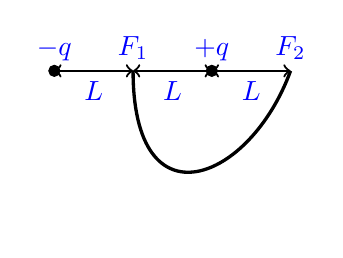
\begin{tikzpicture}
    \draw[fill=black] (0,0) circle (0.07cm) node[above,blue] {$-q$} ;
    \draw[fill=black] (2,0) circle (0.07cm) node[above,blue] {$+q$} ;
    \draw[very thick] (1,0) node[blue,above] {$F_1$} to
    [controls=+(-90:2cm) and +(250:1.5cm)] (3,0) node[blue,above]
    {$F_2$};  
    \draw[thick,<->] (0,0) -- (1,0) node[midway,below,blue] {$L$};
    \draw[thick,<->] (1,0) -- (2,0) node[midway,below,blue] {$L$}; 
    \draw[thick,<->] (2,0) -- (3,0) node[midway,below,blue] {$L$}; 
  \end{tikzpicture}
\end{center}

% Город СПб, 2006, 10 класс


\taskpic{ Верёвка длиной $l$ закреплена одним из своих концов в
  вершине сферы радиуса $R$. В некоторый момент верёвку
  отпускают. Найдите ускорение верёвки сразу после этого. Трение
  отсутствует.   }
{
  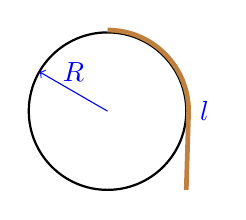
\begin{tikzpicture}
    \draw[thick] (2,2) circle (1cm);
    \draw[line width=0.06cm,brown] (2,3.03) arc (90:0:1.03cm)
    node[right,blue] {$l$};
    \draw[line width=0.06cm,brown] (3.03,2) -- (3,1);
    \draw[->,blue] (2,2) -- ++(150:1cm) node[midway,above] {$R$};
  \end{tikzpicture}
}
% Квант, Ф1273, 1991-6

\task{ Электрический заряд $Q$ равномерно распределён по тонкой
  абсолютно жёсткой металлической сфере радиуса $R$. Какая сила $F$
  действует на единицу площади поверхности со стороны остального
  заряда? }

\task{ Жидкость с диэлектрической проницаемостью $\eps$ налита в
  большой сосуд. Две вертикально расположенные параллельные пластины
  касаются поверхности жидкости. Расстояние между пластинами равно
  $d$. Пластины подключают к источнику с разностью потенциалов
  $U$. Какова будет высота $h$ столба жидкости между пластинами после
  установления равновесия? Плотность жидкости равна $\rho$. }


\task{ Один конец однородной цепочки массы $M$ и длиной $L$ закреплён
  в лапке штатива. При этом вся цепочка повисла, вытянувшись в
  вертикальном направлении и не касаясь пола. Затем другой её конец
  подняли над местом закрепления первого конца на высоту $H<L$ и
  начали медленно перемещать в горизонтальном направлении до тех пор,
  пока касательная к цепочке вблизи её закреплённого конца не стала
  горизонтальной. Какова сила натяжения цепочки вблизи её нижнего
  конца?}

% Квант, 2012-04


\end{document}


%%% Local Variables: 
%%% mode: latex
%%% TeX-engine:xetex
%%% TeX-PDF-mode: t
%%% End:
